\chapter{Hashmap Results}
\label{app:hashmaps}

All results presented are the median of 5 trials. If there is an error bar, the bar represents the maximum and minimum value of the 5 trials.
Cache misses are recorded by evaluating the Multi-Thread Singletons Test with 8 threads, with each thread running 9M transactions, under the profiling tool Performance Events for Linux (\texttt{perf}). The sampling period is set to 1000, meaning that every 1000th cache miss is recorded.
In the figures below, we report the number of cache misses reported by perf (approximately 1/1000 of the actual number of cache misses.)

\section{Multi-Thread Singleton Test Results: 33\% Find, 33\% Insert, 33\% Erase}

\subsection{Cache Misses}
\label{app:hm_cm_33}
    \begin{figure}[H]
    \centering
        {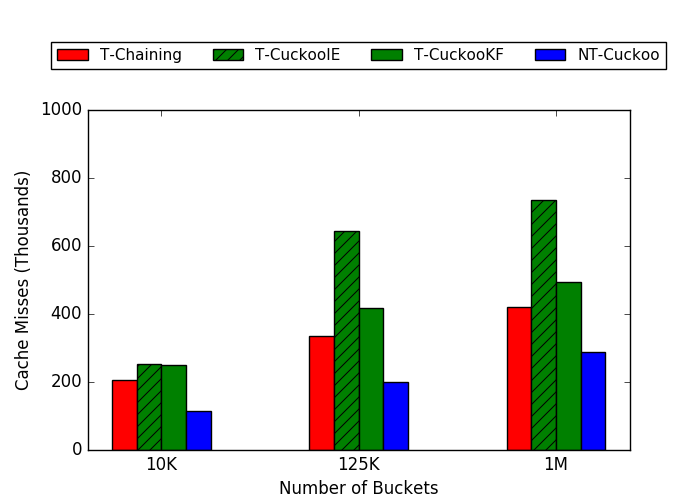
\includegraphics[width=0.45\textwidth]{maps/335cm.png}}
        \caption{Hashmap Cache Misses: Maximum Fullness 5}
    \end{figure}

    \begin{figure}[H]
    \centering
        {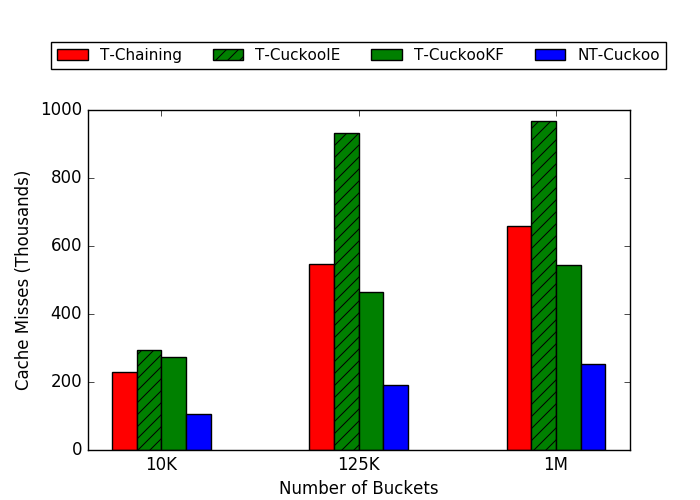
\includegraphics[width=0.45\textwidth]{maps/3310cm.png}}
        \caption{Hashmap Cache Misses: Maximum Fullness 10}
    \end{figure}

    \begin{figure}[H]
    \centering
        {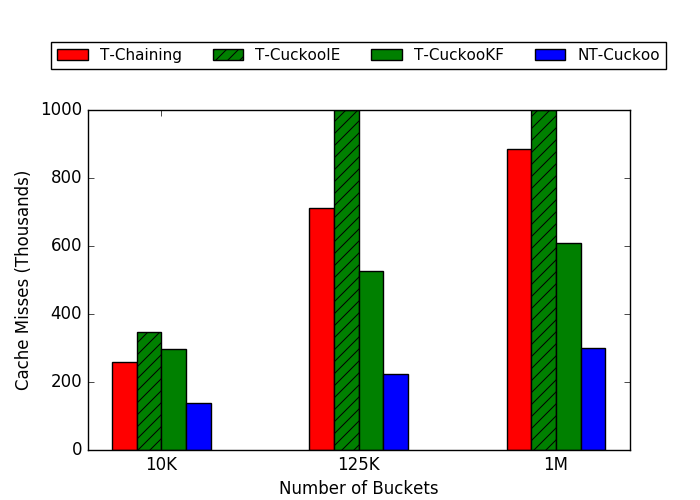
\includegraphics[width=0.45\textwidth]{maps/3315cm.png}}
        \caption{Hashmap Cache Misses: Maximum Fullness 15}
    \end{figure}

\subsection{Maximum Fullness 5}

\begin{figure}[H]
    \centering
	\begin{minipage}{0.5\textwidth}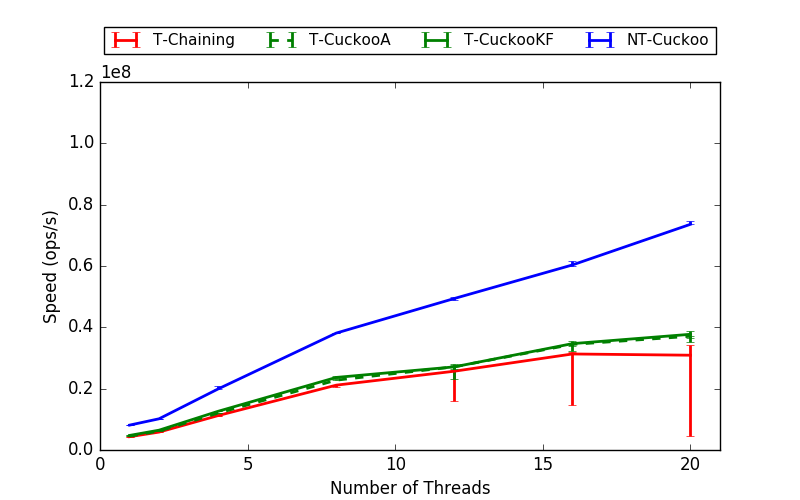
\includegraphics[width=\textwidth]{maps/5HM10K:F34,I33,E33.png} 
    \end{minipage}
	\begin{minipage}{0.4\textwidth}
    \begin{tabular}{|c|c|c|c|}
\hline
\multirow{2}{*}{Hashmap} & \multicolumn{3}{c|}{\#Threads}\\\cline{2-4}& 4 & 12 & 20\\
\hline
\hline
T-Chaining & 0.00325 & 0.01291 & 0.01843\\
T-CuckooA & 0.00108 & 0.00487 & 0.00773\\
T-CuckooKF & 0.00100 & 0.00483 & 0.00799\\
NT-Cuckoo & 0.00000 & 0.00000 & 0.00000\\
\hline
\end{tabular}

    \end{minipage}
    \caption{Hashmap Performance (33F/33I/33E): 10K Buckets, Maximum Fullness 5}
\end{figure}

\begin{figure}[H]
    \centering
	\begin{minipage}{0.5\textwidth}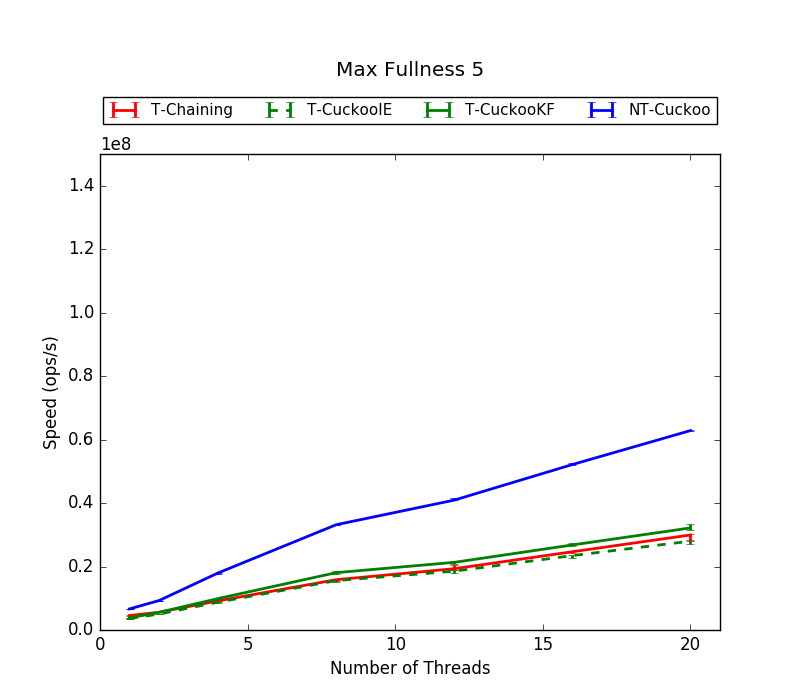
\includegraphics[width=\textwidth]{maps/5HM125K:F34,I33,E33.png} 
    \end{minipage}
	\begin{minipage}{0.4\textwidth}
    \begin{tabular}{|c|c|c|c|}
\hline
\multirow{2}{*}{Hashmap} & \multicolumn{3}{c|}{\#Threads Abort Rate (\%)}\\\cline{2-4}& 4 & 12 & 20\\
\hline
\hline
T-Chaining & 0.000 & 0.001 & 0.002\\
T-CuckooIE & 0.000 & 0.001 & 0.001\\
T-CuckooKF & 0.000 & 0.000 & 0.001\\
NT-Cuckoo & 0.000 & 0.000 & 0.000\\
\hline
\end{tabular}

    \end{minipage}
    \caption{Hashmap Performance (33F/33I/33E): 125K Buckets, Maximum Fullness 5}
\end{figure}

\begin{figure}[H]
    \centering
	\begin{minipage}{0.5\textwidth}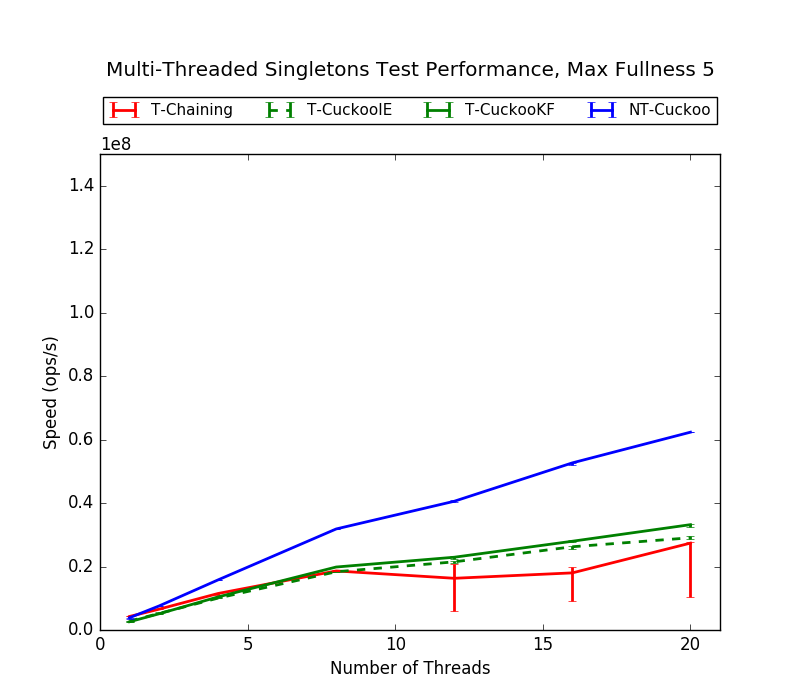
\includegraphics[width=\textwidth]{maps/5HM1M:F34,I33,E33.png} 
    \end{minipage}
	\begin{minipage}{0.4\textwidth}
    \begin{tabular}{|c|c|c|c|c|c|c|}
\hline
\multirow{2}{*}{Hashmap} & \multicolumn{6}{c|}{\#Threads}\\\cline{2-7}& 2 & 4 & 8 & 12 & 16 & 20\\
\hline
\hline
T-Chaining & 0.00002 & 0.00004 & 0.00009 & 0.00012 & 0.00018 & 0.00022\\
T-CuckooA & 0.00000 & 0.00001 & 0.00003 & 0.00004 & 0.00007 & 0.00010\\
T-CuckooKF & 0.00000 & 0.00001 & 0.00002 & 0.00004 & 0.00006 & 0.00009\\
NT-Cuckoo & 0.00000 & 0.00000 & 0.00000 & 0.00000 & 0.00000 & 0.00000\\
\hline
\end{tabular}

    \end{minipage}
    \caption{Hashmap Performance (33F/33I/33E): 1M Buckets, Maximum Fullness 5}
\end{figure}

\subsection{Maximum Fullness 10}

\begin{figure}[H]
    \centering
	\begin{minipage}{0.5\textwidth}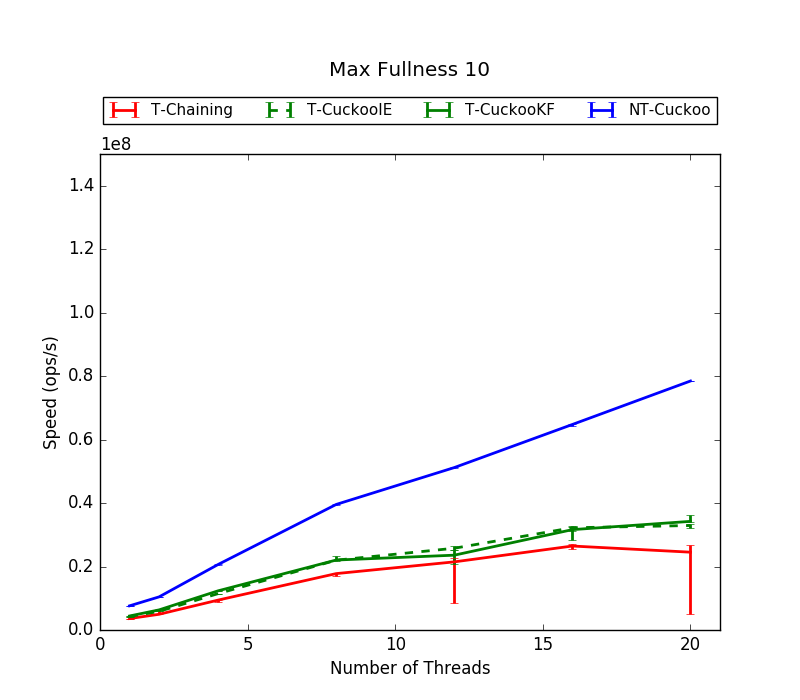
\includegraphics[width=\textwidth]{maps/10HM10K:F34,I33,E33.png} 
    \end{minipage}
	\begin{minipage}{0.4\textwidth}
    \begin{tabular}{|c|c|c|c|}
\hline
\multirow{2}{*}{Hashmap} & \multicolumn{3}{c|}{\#Threads Abort Rate (\%)}\\\cline{2-4}& 4 & 12 & 20\\
\hline
\hline
T-Chaining & 0.003 & 0.013 & 0.021\\
T-CuckooIE & 0.001 & 0.004 & 0.005\\
T-CuckooKF & 0.001 & 0.004 & 0.007\\
NT-Cuckoo & 0.000 & 0.000 & 0.000\\
\hline
\end{tabular}

    \end{minipage}
    \caption{Hashmap Performance (33F/33I/33E): 10K Buckets, Maximum Fullness 10}
\end{figure}

\begin{figure}[H]
    \centering
	\begin{minipage}{0.5\textwidth}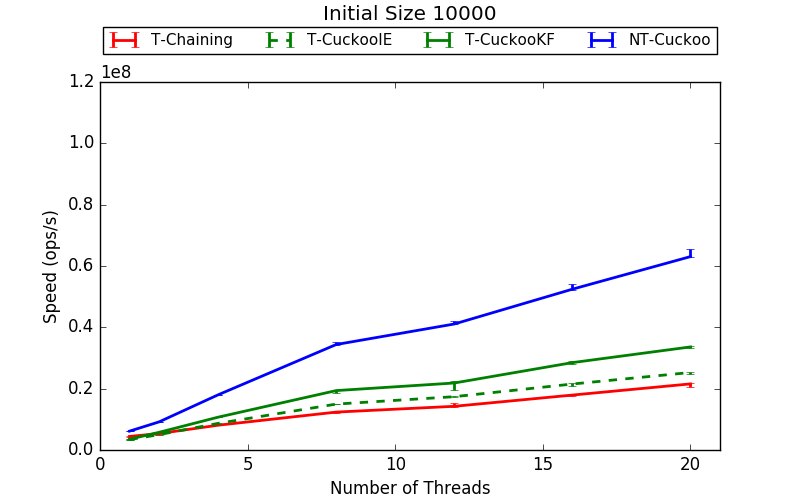
\includegraphics[width=\textwidth]{maps/10HM125K:F34,I33,E33.png} 
    \end{minipage}
	\begin{minipage}{0.4\textwidth}
    \begin{tabular}{|c|c|c|c|}
\hline
\multirow{2}{*}{Hashmap} & \multicolumn{3}{c|}{\#Threads}\\\cline{2-4}& 4 & 12 & 20\\
\hline
\hline
T-Chaining & 0.000 & 0.002 & 0.002\\
T-CuckooIE & 0.000 & 0.000 & 0.001\\
T-CuckooKF & 0.000 & 0.000 & 0.001\\
NT-Cuckoo & 0.000 & 0.000 & 0.000\\
\hline
\end{tabular}

    \end{minipage}
    \caption{Hashmap Performance (33F/33I/33E): 125K Buckets, Maximum Fullness 10}
\end{figure}

\begin{figure}[H]
    \centering
	\begin{minipage}{0.5\textwidth}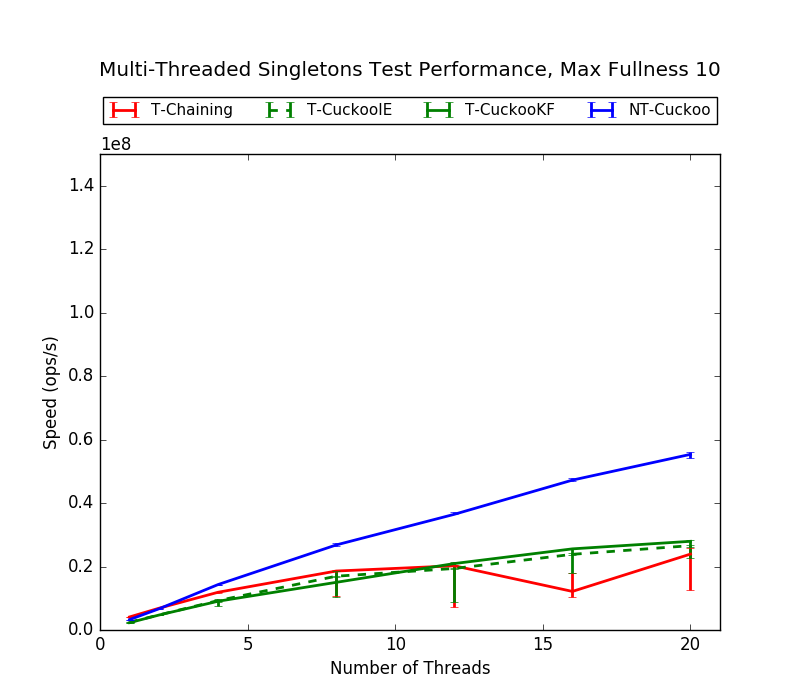
\includegraphics[width=\textwidth]{maps/10HM1M:F34,I33,E33.png} 
    \end{minipage}
	\begin{minipage}{0.4\textwidth}
    \begin{tabular}{|c|c|c|c|}
\hline
\multirow{2}{*}{Hashmap} & \multicolumn{3}{c|}{\#Threads}\\\cline{2-4}& 4 & 12 & 20\\
\hline
\hline
T-Chaining & 0.00004 & 0.34599 & 0.13496\\
T-CuckooA & 0.00001 & 0.15493 & 0.04467\\
T-CuckooKF & 0.00001 & 0.09270 & 0.06208\\
NT-Cuckoo & 0.00000 & 0.00000 & 0.00000\\
\hline
\end{tabular}

    \end{minipage}
    \caption{Hashmap Performance (33F/33I/33E): 1M Buckets, Maximum Fullness 10}
\end{figure}

\subsection{Maximum Fullness 15}

\begin{figure}[H]
    \centering
	\begin{minipage}{0.5\textwidth}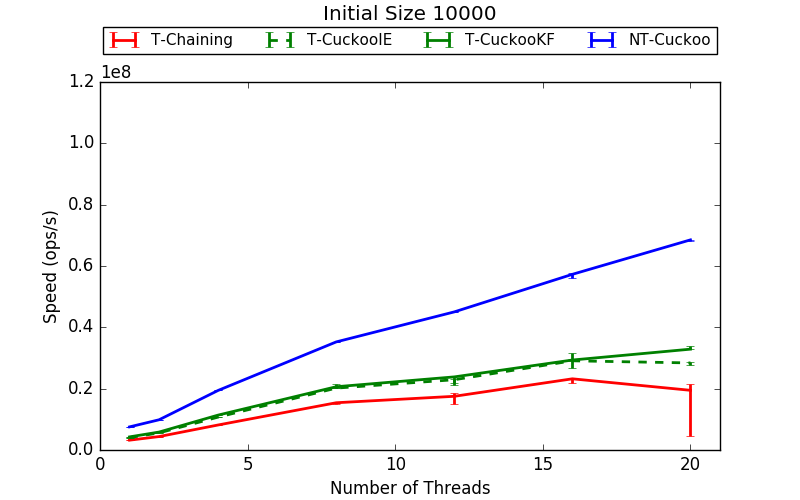
\includegraphics[width=\textwidth]{maps/15HM10K:F34,I33,E33.png} 
    \end{minipage}
	\begin{minipage}{0.4\textwidth}
    \begin{tabular}{|c|c|c|c|}
\hline
\multirow{2}{*}{Hashmap} & \multicolumn{3}{c|}{\#Threads}\\\cline{2-4}& 4 & 12 & 20\\
\hline
\hline
T-Chaining & 0.004 & 0.015 & 0.023\\
T-CuckooIE & 0.001 & 0.004 & 0.005\\
T-CuckooKF & 0.001 & 0.003 & 0.005\\
NT-Cuckoo & 0.000 & 0.000 & 0.000\\
\hline
\end{tabular}

    \end{minipage}
    \caption{Hashmap Performance (33F/33I/33E): 10K Buckets, Maximum Fullness 15}
\end{figure}

\begin{figure}[H]
    \centering
	\begin{minipage}{0.5\textwidth}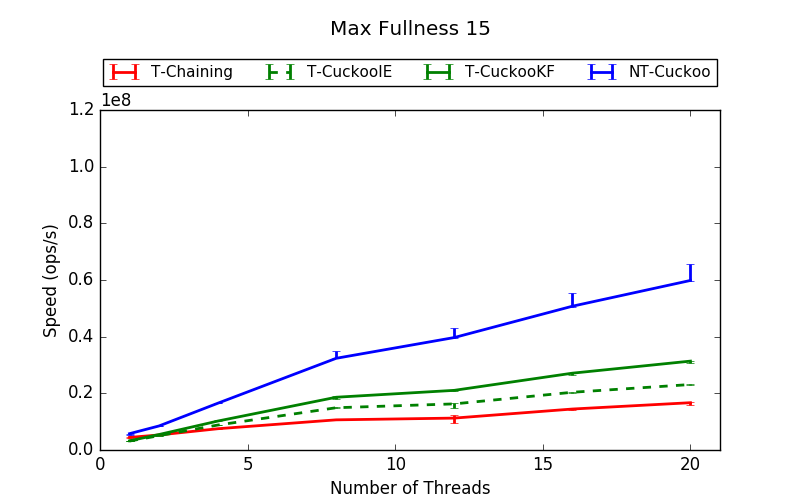
\includegraphics[width=\textwidth]{maps/15HM125K:F34,I33,E33.png} 
    \end{minipage}
	\begin{minipage}{0.4\textwidth}
    \begin{tabular}{|c|c|c|c|}
\hline
\multirow{2}{*}{Hashmap} & \multicolumn{3}{c|}{\#Threads Abort Rate (\%)}\\\cline{2-4}& 4 & 12 & 20\\
\hline
\hline
T-Chaining & 0.000 & 0.002 & 0.003\\
T-CuckooIE & 0.000 & 0.001 & 0.001\\
T-CuckooKF & 0.000 & 0.000 & 0.001\\
NT-Cuckoo & 0.000 & 0.000 & 0.000\\
\hline
\end{tabular}

    \end{minipage}
    \caption{Hashmap Performance (33F/33I/33E): 125K Buckets, Maximum Fullness 15}
\end{figure}

\begin{figure}[H]
    \centering
	\begin{minipage}{0.5\textwidth}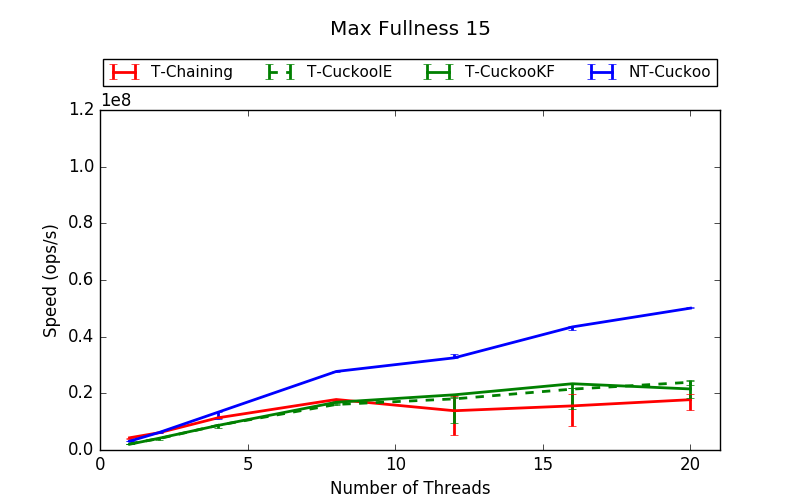
\includegraphics[width=\textwidth]{maps/15HM1M:F34,I33,E33.png} 
    \end{minipage}
	\begin{minipage}{0.4\textwidth}
    \begin{tabular}{|c|c|c|c|c|c|c|}
\hline
\multirow{2}{*}{Hashmap} & \multicolumn{6}{c|}{\#Threads}\\\cline{2-7}& 2 & 4 & 8 & 12 & 16 & 20\\
\hline
\hline
T-Chaining & 0.00002 & 0.00005 & 0.14779 & 0.08940 & 0.00022 & 0.00027\\
T-CuckooA & 0.00000 & 0.00001 & 0.03164 & 0.01825 & 0.00005 & 0.00008\\
T-CuckooKF & 0.00000 & 0.00001 & 0.01399 & 0.00735 & 0.00005 & 0.00007\\
NT-Cuckoo & 0.00000 & 0.00000 & 0.00000 & 0.00000 & 0.00000 & 0.00000\\
\hline
\end{tabular}

    \end{minipage}
    \caption{Hashmap Performance (33F/33I/33E): 1M Buckets, Maximum Fullness 15}
\end{figure}

\section{Multi-Thread Singleton Test Results: 90\% Find, 5\% Insert, 5\% Erase}

\subsection{Cache Misses}
\label{app:hm_cm_90}
    \begin{figure}[H]
    \centering
        {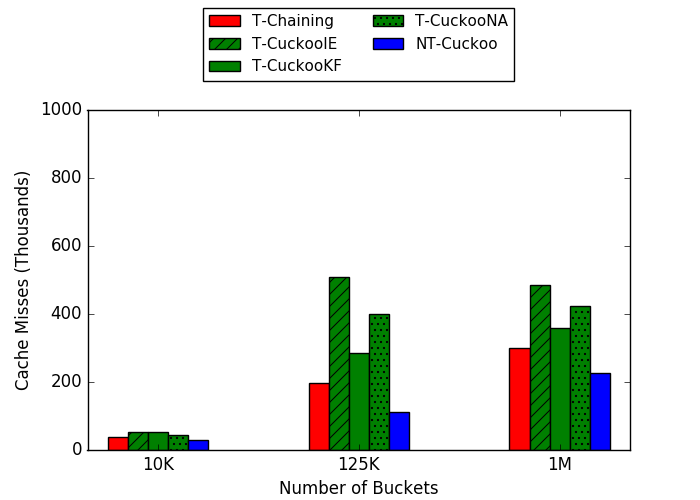
\includegraphics[width=0.45\textwidth]{maps/905cm.png}}
        \caption{Hashmap Cache Misses: Maximum Fullness 5}
    \end{figure}

    \begin{figure}[H]
    \centering
        {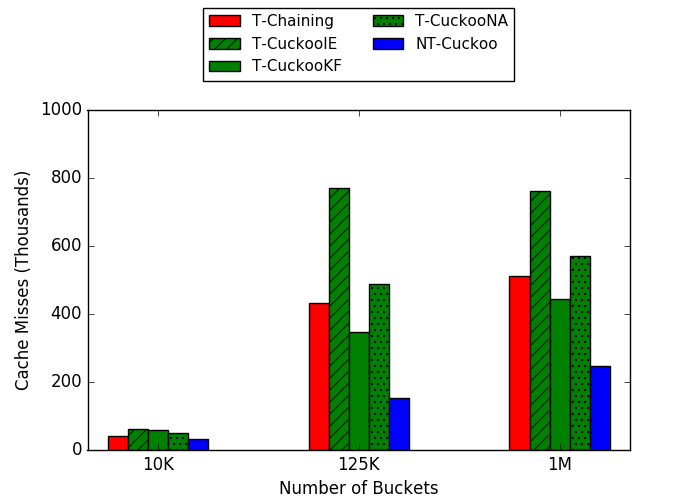
\includegraphics[width=0.45\textwidth]{maps/9010cm.png}}
        \caption{Hashmap Cache Misses: Maximum Fullness 10}
    \end{figure}

    \begin{figure}[H]
    \centering
        {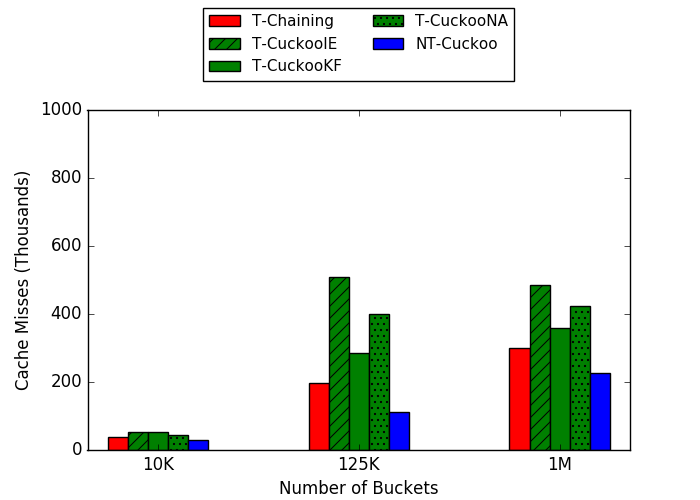
\includegraphics[width=0.45\textwidth]{maps/905cm.png}}
        \caption{Hashmap Cache Misses: Maximum Fullness 15}
    \end{figure}

\subsection{Maximum Fullness 5}

\begin{figure}[H]
    \centering
	\begin{minipage}{0.5\textwidth}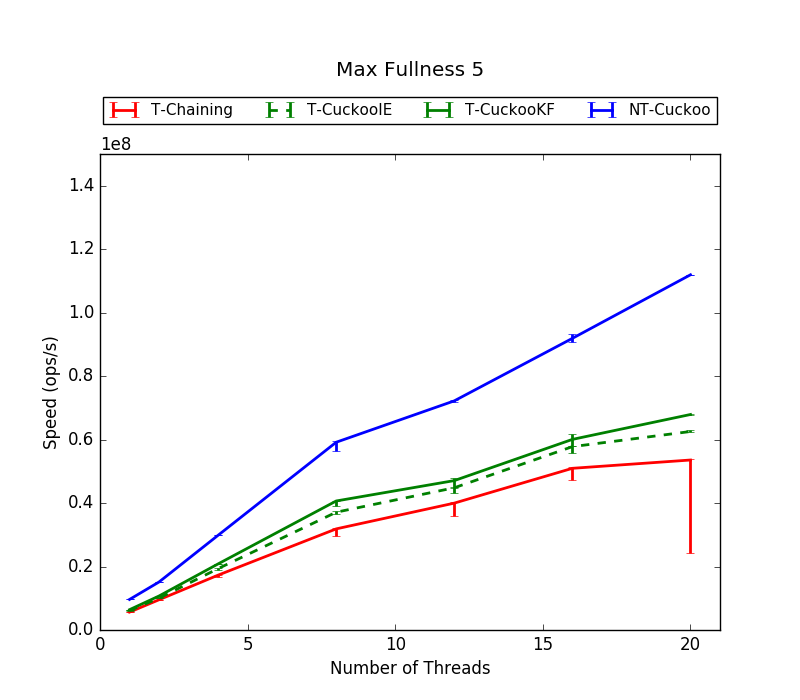
\includegraphics[width=\textwidth]{maps/5HM10K:F90,I5,E5.png} 
    \end{minipage}
	\begin{minipage}{0.4\textwidth}
    \begin{tabular}{|c|c|c|c|}
\hline
\multirow{2}{*}{Hashmap} & \multicolumn{3}{c|}{\#Threads}\\\cline{2-4}& 4 & 12 & 20\\
\hline
\hline
T-Chaining & 0.001 & 0.003 & 0.005\\
T-CuckooIE & 0.001 & 0.001 & 0.002\\
T-CuckooKF & 0.000 & 0.001 & 0.002\\
NT-Cuckoo & 0.000 & 0.000 & 0.000\\
\hline
\end{tabular}

    \end{minipage}
    \caption{Hashmap Performance (34F/5I/5E): 10K Buckets, Maximum Fullness 5}
\end{figure}

\begin{figure}[H]
    \centering
	\begin{minipage}{0.5\textwidth}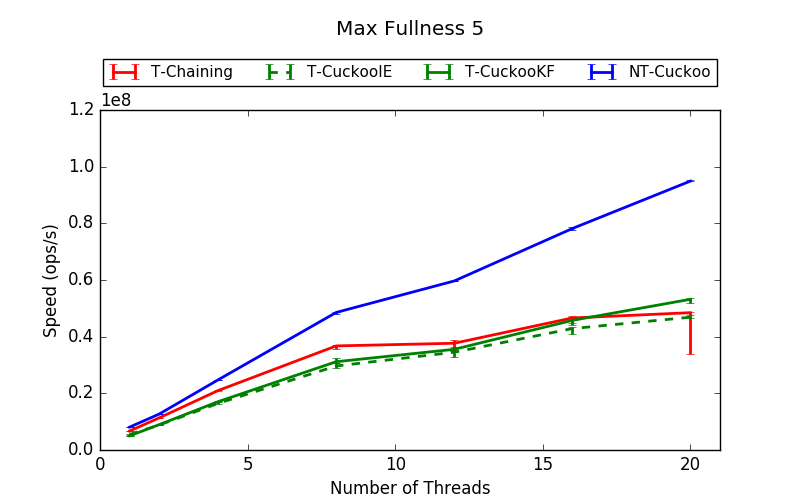
\includegraphics[width=\textwidth]{maps/5HM125K:F90,I5,E5.png} 
    \end{minipage}
	\begin{minipage}{0.4\textwidth}
    \begin{tabular}{|c|c|c|c|}
\hline
\multirow{2}{*}{Hashmap} & \multicolumn{3}{c|}{\#Threads}\\\cline{2-4}& 4 & 12 & 20\\
\hline
\hline
T-Chaining & 0.00006 & 0.00023 & 0.00038\\
T-CuckooA & 0.00003 & 0.00011 & 0.00026\\
T-CuckooKF & 0.00003 & 0.00011 & 0.00026\\
NT-Cuckoo & 0.00000 & 0.00000 & 0.00000\\
\hline
\end{tabular}

    \end{minipage}
    \caption{Hashmap Performance (34F/5I/5E): 125K Buckets, Maximum Fullness 5}
\end{figure}

\begin{figure}[H]
    \centering
	\begin{minipage}{0.5\textwidth}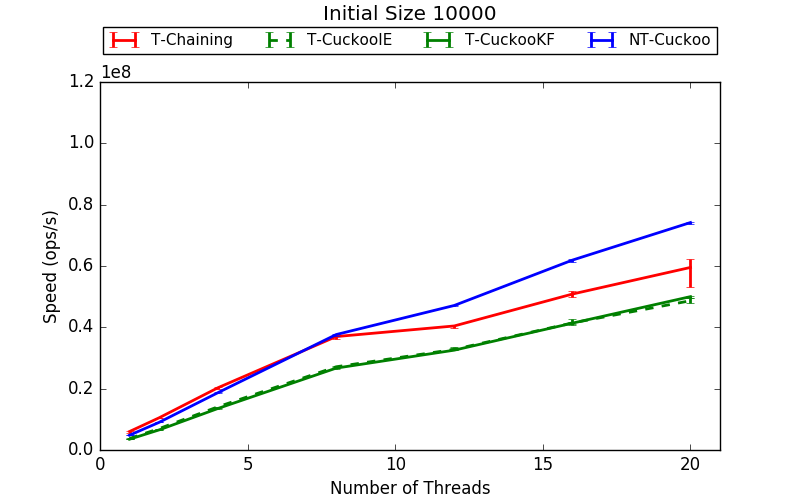
\includegraphics[width=\textwidth]{maps/5HM1M:F90,I5,E5.png} 
    \end{minipage}
	\begin{minipage}{0.4\textwidth}
    \begin{tabular}{|c|c|c|c|}
\hline
\multirow{2}{*}{Hashmap} & \multicolumn{3}{c|}{\#Threads}\\\cline{2-4}& 4 & 12 & 20\\
\hline
\hline
T-Chaining & 0.00001 & 0.00003 & 0.00006\\
T-CuckooA & 0.00001 & 0.00001 & 0.00003\\
T-CuckooKF & 0.00000 & 0.00001 & 0.00003\\
NT-Cuckoo & 0.00000 & 0.00000 & 0.00000\\
\hline
\end{tabular}

    \end{minipage}
    \caption{Hashmap Performance (34F/5I/5E): 1M Buckets, Maximum Fullness 5}
\end{figure}

\subsection{Maximum Fullness 10}

\begin{figure}[H]
    \centering
	\begin{minipage}{0.5\textwidth}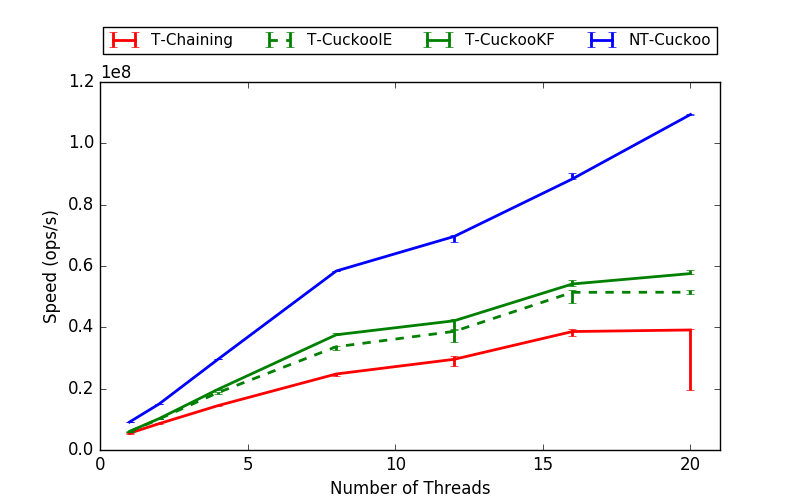
\includegraphics[width=\textwidth]{maps/10HM10K:F90,I5,E5.png} 
    \end{minipage}
	\begin{minipage}{0.4\textwidth}
    \begin{tabular}{|c|c|c|c|c|c|c|}
\hline
\multirow{2}{*}{Hashmap} & \multicolumn{6}{c|}{\#Threads}\\\cline{2-7}& 2 & 4 & 8 & 12 & 16 & 20\\
\hline
\hline
T-Chaining & 0.00050 & 0.00100 & 0.00229 & 0.00318 & 0.00409 & 0.00534\\
T-CuckooA & 0.00020 & 0.00057 & 0.00106 & 0.00150 & 0.00178 & 0.00233\\
T-CuckooKF & 0.00020 & 0.00057 & 0.00095 & 0.00140 & 0.00171 & 0.00243\\
NT-Cuckoo & 0.00000 & 0.00000 & 0.00000 & 0.00000 & 0.00000 & 0.00000\\
\hline
\end{tabular}

    \end{minipage}
    \caption{Hashmap Performance (90F/5I/5E): 10K Buckets, Maximum Fullness 10}
\end{figure}

\begin{figure}[H]
    \centering
	\begin{minipage}{0.5\textwidth}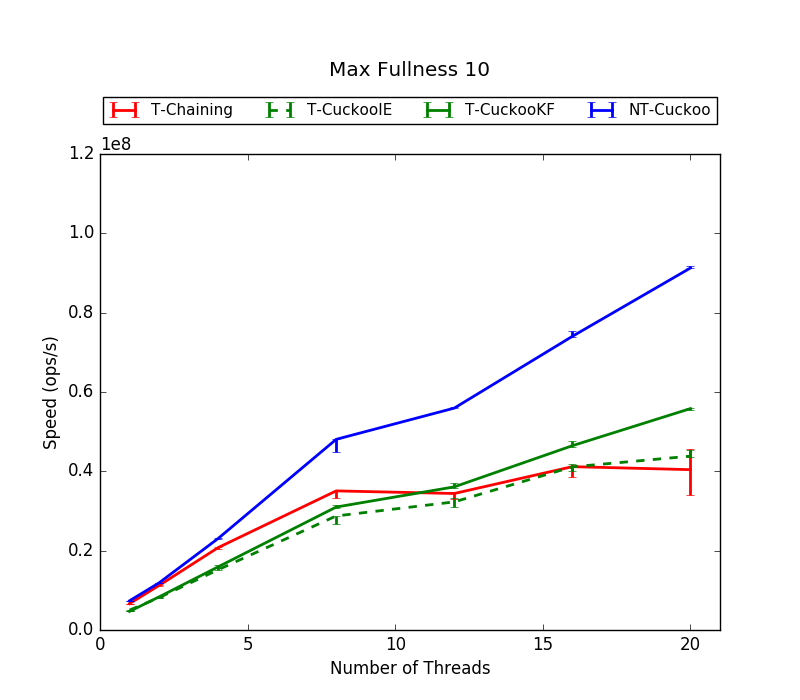
\includegraphics[width=\textwidth]{maps/10HM125K:F90,I5,E5.png} 
    \end{minipage}
	\begin{minipage}{0.4\textwidth}
    \begin{tabular}{|c|c|c|c|c|c|c|}
\hline
\multirow{2}{*}{Hashmap} & \multicolumn{6}{c|}{Number of Threads Abort Rate (\%)}\\\cline{2-7}& 2 & 4 & 8 & 12 & 16 & 20\\
\hline
\hline
T-Chaining & 0.000 & 0.000 & 0.000 & 0.000 & 0.001 & 0.001\\
T-CuckooIE & 0.000 & 0.000 & 0.000 & 0.000 & 0.000 & 0.001\\
T-CuckooKF & 0.000 & 0.000 & 0.000 & 0.000 & 0.000 & 0.001\\
NT-Cuckoo & 0.000 & 0.000 & 0.000 & 0.000 & 0.000 & 0.000\\
\hline
\end{tabular}

    \end{minipage}
    \caption{Hashmap Performance (90F/5I/5E): 125K Buckets, Maximum Fullness 10}
\end{figure}

\begin{figure}[H]
    \centering
	\begin{minipage}{0.5\textwidth}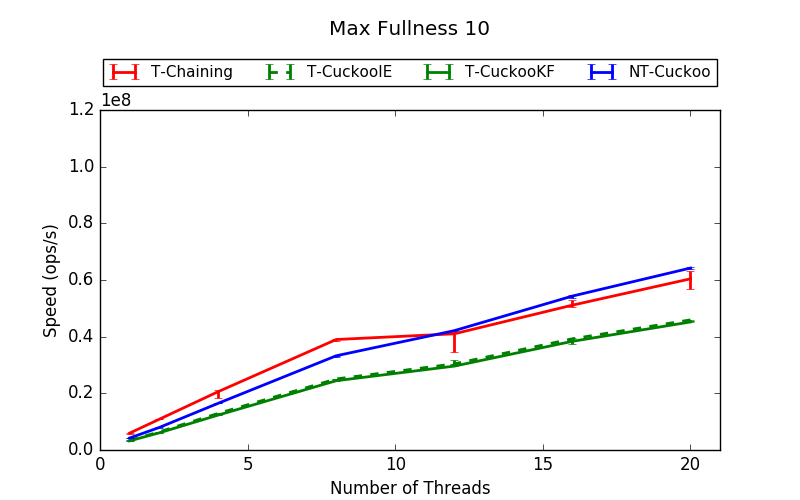
\includegraphics[width=\textwidth]{maps/10HM1M:F90,I5,E5.png} 
    \end{minipage}
	\begin{minipage}{0.4\textwidth}
    \begin{tabular}{|c|c|c|c|}
\hline
\multirow{2}{*}{Hashmap} & \multicolumn{3}{c|}{\#Threads}\\\cline{2-4}& 4 & 12 & 20\\
\hline
\hline
T-Chaining & 0.00001 & 0.00034 & 0.00022\\
T-CuckooA & 0.00000 & 0.00050 & 0.00007\\
T-CuckooKF & 0.00000 & 0.00026 & 0.00003\\
NT-Cuckoo & 0.00000 & 0.00000 & 0.00000\\
\hline
\end{tabular}

    \end{minipage}
    \caption{Hashmap Performance (90F/5I/5E): 1M Buckets, Maximum Fullness 10}
\end{figure}

\subsection{Maximum Fullness 15}

\begin{figure}[H]
    \centering
	\begin{minipage}{0.5\textwidth}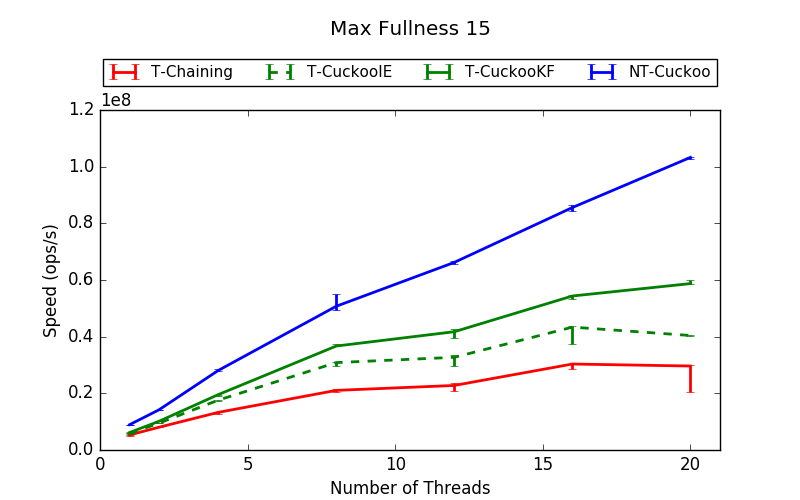
\includegraphics[width=\textwidth]{maps/15HM10K:F90,I5,E5.png} 
    \end{minipage}
	\begin{minipage}{0.4\textwidth}
    \begin{tabular}{|c|c|c|c|c|c|c|}
\hline
\multirow{2}{*}{Hashmap} & \multicolumn{6}{c|}{\#Threads}\\\cline{2-7}& 2 & 4 & 8 & 12 & 16 & 20\\
\hline
\hline
T-Chaining & 0.00030 & 0.00103 & 0.00266 & 0.00378 & 0.00449 & 0.00584\\
T-CuckooA & 0.00025 & 0.00065 & 0.00115 & 0.00166 & 0.00205 & 0.00250\\
T-CuckooKF & 0.00010 & 0.00068 & 0.00111 & 0.00163 & 0.00196 & 0.00262\\
NT-Cuckoo & 0.00000 & 0.00000 & 0.00000 & 0.00000 & 0.00000 & 0.00000\\
\hline
\end{tabular}

    \end{minipage}
    \caption{Hashmap Performance (90F/5I/5E): 10K Buckets, Maximum Fullness 15}
\end{figure}

\begin{figure}[H]
    \centering
	\begin{minipage}{0.5\textwidth}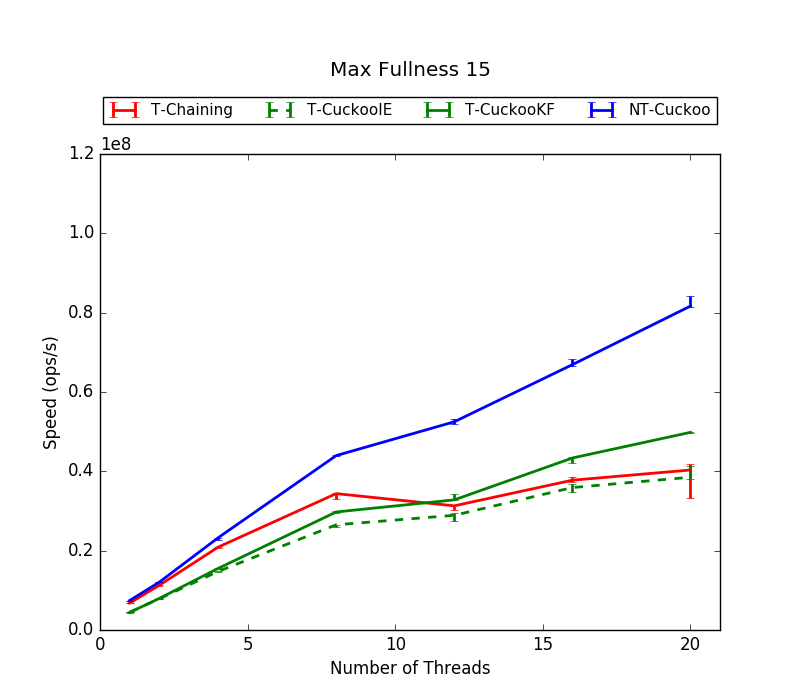
\includegraphics[width=\textwidth]{maps/15HM125K:F90,I5,E5.png} 
    \end{minipage}
	\begin{minipage}{0.4\textwidth}
    \begin{tabular}{|c|c|c|c|}
\hline
\multirow{2}{*}{Hashmap} & \multicolumn{3}{c|}{\#Threads}\\\cline{2-4}& 4 & 12 & 20\\
\hline
\hline
T-Chaining & 0.00009 & 0.00027 & 0.00047\\
T-CuckooA & 0.00004 & 0.00013 & 0.00023\\
T-CuckooKF & 0.00002 & 0.00007 & 0.00018\\
NT-Cuckoo & 0.00000 & 0.00000 & 0.00000\\
\hline
\end{tabular}

    \end{minipage}
    \caption{Hashmap Performance (90F/5I/5E): 125K Buckets, Maximum Fullness 15}
\end{figure}

\begin{figure}[H]
    \centering
	\begin{minipage}{0.5\textwidth}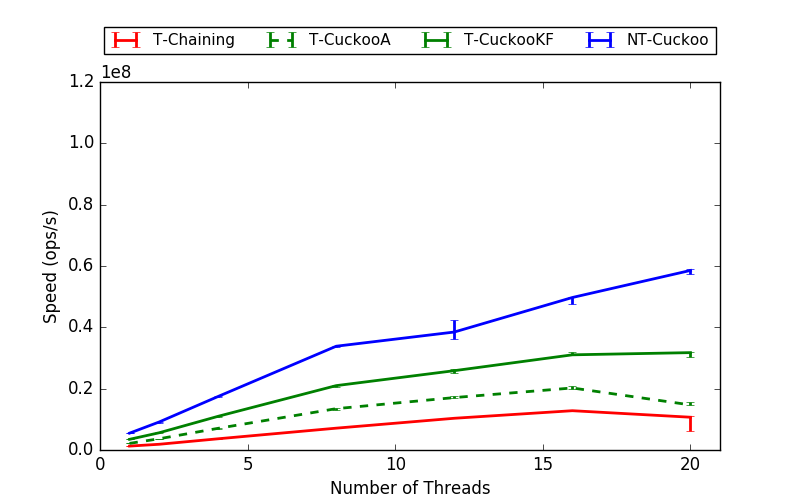
\includegraphics[width=\textwidth]{maps/15HM1M:F90,I5,E5.png} 
    \end{minipage}
	\begin{minipage}{0.4\textwidth}
    \begin{tabular}{|c|c|c|c|}
\hline
\multirow{2}{*}{Hashmap} & \multicolumn{3}{c|}{\#Threads}\\\cline{2-4}& 4 & 12 & 20\\
\hline
\hline
T-Chaining & 0.00001 & 0.00636 & 0.00016\\
T-CuckooA & 0.00000 & 0.00001 & 0.00037\\
T-CuckooKF & 0.00000 & 0.00001 & 0.00006\\
NT-Cuckoo & 0.00000 & 0.00000 & 0.00000\\
\hline
\end{tabular}

    \end{minipage}
    \caption{Hashmap Performance (90F/5I/5E): 1M Buckets, Maximum Fullness 15}
\end{figure}

\iffalse
\begin{table}[H]
    \centering
\begin{tabular}{|c|c|c|c|c|c|}
    find(x)-find(x) & insert(x)-insert(x) & erase(x)-erase(x) & find(x)-insert(x) & find(x)-erase(x) & insert(x)-erase(x)\\
    \hline
    & W-W, W-R & W-W, W-R & R-W & R-W & W-W, W-R
\end{tabular}
    \caption*{R-R relations are not shown.}
    \caption{Dependencies of pairs of hashmap operations}
    \label{table:hashmapsimpledeps}
\end{table}
\fi
